\chapter{绪论}
\label{chap:introduction}

\section{研究背景和意义}
点云(Point Cloud)是一种高效的三维对象表达方式。点云是由一组点构成的集合,每个点由其三维坐标$(x,y,z)$和可能的其他属性(如颜色信息或者法线方向)组成。
%由于点云能够高效地表示三维空间中的任意形状,所以点云被广泛应用于各个领域。同时,随着深度传感器技术的发展,例如微软的Kinect深度相机、LiDAR 三维扫描仪、光场相机、智能手机搭载的结构光传感器等能够方便地采集三维点云数据,点云数据的应用前景巨大。但同时缺少高效、灵活的点云处理技术,因此,越来越多的点云数据亟待被识别加以利用,将点云处理的结果应用于各种实际应用场景中去,点云识别技术成为了一个具有巨大研究价值和应用前景的学科方向,例如点云的分类、分割技术等是目前活跃的研究课题。点云数据一般被认为是非欧氏数据(Non-Euclidean data)。传统的深度学习技术大多数基于结构化数据,故大多数先前的利用卷积神经网络来对点云进行识别的工作,多将点云数据转化为多视角的二维图像或对点云进行体素化,把点云数据转化为某种规则的结构化数据,再输入网络进行学习。然而,对点云进行这样的转化会产生大量的临时数据并会引入量化误差,所以如让神经网络处理原始点云数据成为了一个研究热点。相较于具有网格结构的欧式数据,点云具有旋转不变性、尺度不变性、顺序不变性、平移不变性等特点\cite{wang2019dynamic},标准卷积网络无法克服这些问题,所以如何解决点云数据存在的这些问题,成为了将深度学习技术应用于点云识别的一大障碍,同时也是目前几何深度学习(Geometric Learning)的研究热点。
公式测试:
\begin{equation}
	h^{l+1} = \sum_i {e_i - e_j}
\end{equation}

\begin{equation}
	max\sum_{i \in \Omega_t^{load} }\sum_{j \in \Omega_t^{FD} }w_{ij,t}x_{ij,t}P_{ij,t}^{La}
\end{equation}

内联公式测试$N_i = \{  N_{ij}^{P}\}$

\subsection{}
%\begin{figure}[htbp]
%\centering
%\subfigure[心脏电影(一帧)]{
%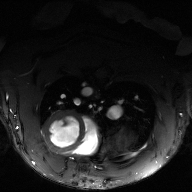
\includegraphics[width=2.11in]{img/intro/cine.png}
%}
%\subfigure[胸部DCE-MRI(一帧)]{
%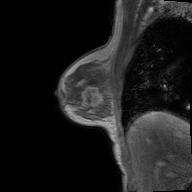
\includegraphics[width=2.11in]{img/intro/breast.png}
%}
%\subfigure[心脏灌注(一帧)]{
%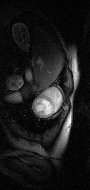
\includegraphics[width=1in]{img/intro/perfusion.png}
%}
%\centering
%\caption{动态MR图像举例。}
%\label{fig:dynamic}
%\end{figure}

\section{本文的主要研究内容和章节安排}

针对xxx存在的问题,本文提出xxx。

第二章 ...

第三章 ...

第四章 ...

第五章,我们对本文的工作进行了总结并给出了下一步工作展望。





